% ======================================================================
\subsection{The global attractor}

% ----------------------------------------------------------------------
\begin{frame}[shrink]%[allowframebreaks]
  \frametitle{The global attractor}

  \setbeamercolor{block title}{fg=white, bg=green!75!black}
  \begin{block}{Definition}
    The global attractor $\mathcal{A}$ is
    the maximal compact invariant set
    \begin{equation}
      S(t)\mathcal{A} = \mathcal{A} \quad \text{for all} \quad
      t \ge 0
      \label{eq:ga1}
    \end{equation}
    and the minimal set that attracts all bounded sets:
    \begin{equation}
      \dist(S(t)X, A) \to 0 \quad \text{as} \quad t\to\infty
      \label{eq:ga2}
    \end{equation}
    for any bounded set $X\subset \pS$. $\pS$ is the phase space.
    $S(t)$ is the semigroup $S(t)\ssp_0 = \ssp(t)$.
  \end{block}

  \pause

  \[
    \omega(X) = \{y :
    \text{there exist sequences}\; t_n\to\infty\;\text{and}\; \ssp_n\in X \;
    \text{with}\; S(t_n)\ssp_n\to y\}
    \,.
  \]
  \begin{block}{Theorem}
    If $S(t)$ is dissipative and $B\subset \pS$ is a compact absorbing
    set then there exists a global attractor $\mathcal{A} = \omega(B)$.
  \end{block}

\end{frame}


% ----------------------------------------------------------------------
\begin{frame}[shrink]%[allowframebreaks]
  \frametitle{An example}

  \begin{figure}[h]
    \centering
    (a)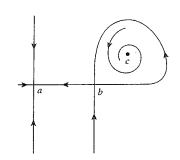
\includegraphics[width=0.4\textwidth]{attractor_portrait_2dsystem}
    (b)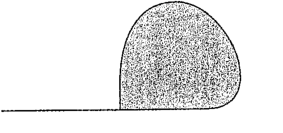
\includegraphics[width=0.5\textwidth]{attractor_2dsystem}
    \caption[The global attractor of a 2d system]{
      (a) Phase portrait of a 2d system.
      (b) The corresponding global attractor.
      (\cite{Robinson2001}).
    }
    \label{fig:attractor_portrait}
  \end{figure}
  {$\mathcal{A} = \omega(B)$.}
  \[
    \omega(X) = \{y :
    \text{there exist sequences}\; t_n\to\infty\;\text{and}\; x_n\in X \;
    \text{with}\; S(t_n)x_n\to y\}
    \,.
  \]

  \pause

  The global attractor:

  {\color{blue} 3 equilibria $\{a, b, c\}$ },
  {\color{cyan} the stable manifold of $c$ },
  {\color{blue} the homoclinic orbit of $b$},
  {\color{cyan} the   heteroclinic orbit from $b$ to $a$}.


\end{frame}

% ======================================================================
\subsection{The dimension of an attractor}

% ----------------------------------------------------------------------
\begin{frame}[shrink]%[allowframebreaks]
  \frametitle{The dimension of an attractor}

  \setbeamercolor{block title}{fg=white, bg=green!75!black}
  \begin{block}{Box-counting dimension (capacity dimension, Kolmogorov dimension)}
    \[
      D_C = \limsup_{\epsilon \to 0} \frac{\log N(\epsilon)}{\log(1/\epsilon)}
    \]
  \end{block}

  \begin{columns}[C] % contents are top vertically aligned
    \column{0.7\textwidth}

    \begin{figure}[h]
      \centering
      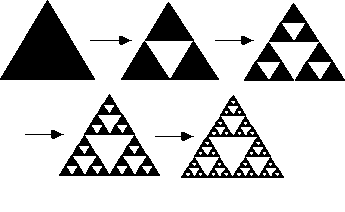
\includegraphics[width=0.5\textwidth]{sierp-det}
      \caption[The Sierpinski striangle]{
        The Sierpinski triangle.
      }
      \label{fig:sier-tri}
    \end{figure}

    \column{0.3\textwidth}
    $D_C = \log 3/ \log 2$.

  \end{columns}

  \pause

  \begin{block}{\small Kaplan-Yorke dimension\cite{KapYor79a, FKYY83}}
    \[
      D_{KY} = k + \frac{\sum_{i=1}^{k} \lambda_i}{|\lambda_{k+1}|}
    \]
    with $k$ the largest number making $\lambda_1 + \cdots + \lambda_k$
    non-negative.
  \end{block}

\end{frame}

% ======================================================================
\subsection{The inertial manifold}

% ----------------------------------------------------------------------
\begin{frame}[shrink]%[allowframebreaks]
  \frametitle{The inertial manifold\cite{Foias1988a, Robinson1995}}

  \setbeamercolor{block title}{fg=white, bg=green!75!black}
  \begin{block}{definition}
    An inertial manifold $\mathcal{I}$ is a finite-dimensional Lipschitz manifold,
    which is positively invariant and attracts all trajectories exponentially,
    \begin{equation}
      \label{eq:im_def}
      \dist(S(t)u_0, \mathcal{M}) \le C(|u_0|)e^{-kt}\quad
      \text{for some } k > 0 \text{ and all } u_0 \in \pS
    \end{equation}
  \end{block}

  \begin{equation}
    \label{eq:proto}
    \frac{du}{dt} + Au + f(u) = 0
    \,.
  \end{equation}

  \begin{equation}
    \label{eq:pq}
    Q_n = I - P_n\,,\quad p(t) = P_nu(t) \,,\quad q(t) = Q_nu(t)
  \end{equation}
  \begin{equation}
    \label{eq:projected}
    \frac{dp}{dt} + Ap + Pf(p+\Phi(p)) = 0
    \,.
  \end{equation}
  The graph of $\Phi$
  \[
    \mathcal{G}[\Phi] := \{u: u = p + \Phi(p)\,, p\in P_n\pS\}
  \]
  defines an $n$-dimensional manifold.

\end{frame}
